\section{Compression, Prediction and Lossless Coding}




\begin{questionbox}{Domanda 5}
Principles of image compression. Discuss the criteria for evaluating a compression algorithm: \textbf{rate}, quality, [Bonus: robustness, delay, complexity].
\end{questionbox}


Compression reduces the number of bits needed to represent multimedia data by exploiting:

\begin{itemize}
  \item \textbf{Statistical redundancy:} neighboring samples, blocks or frames are correlated.
  \item \textbf{Spatial / temporal redundancy:} images and videos contain repeated structures across space and time.
  \item \textbf{Psychovisual redundancy:} distortions not perceived by the human visual system can be coarsely quantized.
\end{itemize}

Compression can be:

\begin{itemize}
  \item \textbf{\textbf{lossless}:} perfect reconstruction, bit-exact output, lower compression ratio.
  \item \textbf{\textbf{lossy}:} decoded signal differs from the original but is perceptually close, higher compression ratio.
\end{itemize}

\textbf{rate} measures coded size:


$$
R_{\text{image}} = \frac{B_{\text{out}}}{NM} \quad [\text{bpp}]
$$



$$
R_{\text{stream}} = \frac{B_{\text{out}}}{T} \quad [\text{bit/s}]
$$


Compression ratio is:


$$
\text{CR} = \frac{B_{\text{in}}}{B_{\text{out}}}
$$


Quality is usually evaluated by \textbf{distortion} measures:


$$
D(f,\hat{f}) = \frac{1}{NM}\|f-\hat{f}\|^2
$$



$$
\text{PSNR}(f,\hat{f}) = 10\log_{10}\left(\frac{V^2}{D(f,\hat{f})}\right)
$$


For perceptual weighting:


$$
D_W(f,\hat{f}) = \frac{1}{NM}\|h \star (f-\hat{f})\|^2
$$



$$
\text{WPSNR}(f,\hat{f}) = 10\log_{10}\left(\frac{V^2}{D_W(f,\hat{f})}\right)
$$


Other objective metrics are \textbf{\textbf{SSIM}} and \textbf{\textbf{LPIPS}}. The main design tensions are: higher quality usually requires higher \textbf{rate}; robustness, lower delay and lower complexity are often in conflict.



\begin{questionbox}{Domanda 6}
A zero-mean Gaussian random signal \textbf{HAS} an autocorrelation function:
\end{questionbox}

$$
> r_X(n-m)=E[X(n)X(m)] = \sigma^2\rho^{|n-m|}
> $$
> - Consider the predictor $V(n)=X(n-1)$. For which values is the prediction gain positive?
> - Optimal linear predictor is $V(n)=-\sum_{i=1}^{P} a_i x_{n-i}$, with $a=-R_X^{-1}r$, $R_X(i,j)=r_X(i-j)$, $r=[r_X(1)\cdots r_X(P)]^T$. Find optimal linear predictor of order $P=1$ and compute prediction gain, compare then with previous case.
> - Compute the optimal predictor of order 2. Compare with the previous cases.

Let:


$$
r_X(n-m)=\mathbb{E}[X(n)X(m)] = \sigma^2\rho^{|n-m|}
$$


For the predictor $V(n)=X(n-1)$:


$$
\sigma_y^2 = \mathbb{E}[(X(n)-X(n-1))^2] = 2\sigma^2(1-\rho)
$$



$$
G_P = 10\log_{10}\left(\frac{\sigma^2}{\sigma_y^2}\right)
=10\log_{10}\left(\frac{1}{2(1-\rho)}\right)
$$


The gain is positive iff:


$$
\rho > \frac{1}{2}
$$


For the optimal linear predictor:


$$
V(n) = -\sum_{i=1}^{P} a_i x(n-i)
$$


with:


$$
\vec{a}^{\,opt} = -R_X^{-1}\vec{r}
$$


For $P=1$:


$$
a_1^{opt}=-\rho \quad \Rightarrow \quad V(n)=\rho X(n-1)
$$



$$
\sigma_y^2=\sigma^2(1-\rho^2)
$$



$$
G_P = 10\log_{10}\left(\frac{1}{1-\rho^2}\right)
$$


For $P=2$, the autocorrelation matrix is:


$$
R_X = \sigma^2
\begin{bmatrix}
1 & \rho \\
\rho & 1
\end{bmatrix},
\quad
\vec{r} = \sigma^2
\begin{bmatrix}
\rho \\
\rho^2
\end{bmatrix}
$$


and:


$$
\vec{a}^{\,opt} =
\begin{bmatrix}
-\rho \\
0
\end{bmatrix}
$$


Thus the second tap gives no extra gain for an AR(1) source.



\begin{questionbox}{Domanda 7}
Draw and comment on the schemes of \textbf{predictive \textbf{quantization}} (encoder and decoder).
\end{questionbox}


\begin{figure}[H]
\centering
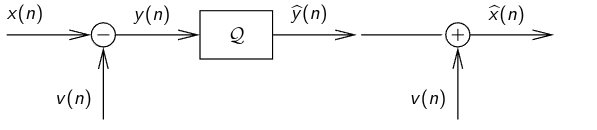
\includegraphics[width=0.75\textwidth]{images/Predictive_quantization_-_open_loop.png}
\caption{Predictive quantization - open loop}
\end{figure}\begin{tcolorbox}[colback=white, colframe=gray!50, height=4.5cm, sharp corners]
\end{tcolorbox}

The open-loop scheme shows the basic \textbf{predictive \textbf{quantization}} idea: the predictor output $v(n)$ is subtracted from the current sample, only the residual $y(n)$ is quantized, and the prediction is added back after \textbf{quantization}. It is useful to understand \textbf{DPCM}-style coding, but it is not safe as a complete codec because the encoder and decoder may base prediction on different past samples.

Open-loop prediction is wrong because the encoder predicts from original samples while the decoder predicts from reconstructed samples. This mismatch causes \textbf{drift}.

Correct \textbf{predictive \textbf{quantization}} uses a closed reconstruction loop at the encoder:

\begin{figure}[H]
\centering
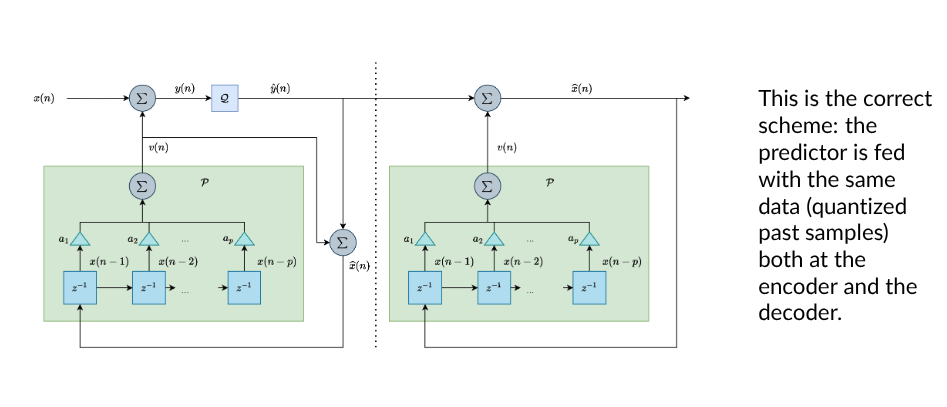
\includegraphics[width=0.75\textwidth]{images/Predictive_quantization_-_correct_closed_loop.png}
\caption{Predictive quantization - correct closed loop}
\end{figure}\begin{tcolorbox}[colback=white, colframe=gray!50, height=4.5cm, sharp corners]
\end{tcolorbox}

The encoder and decoder feed the predictor with the same reconstructed samples:


$$
y(n)=x(n)-v(n)
$$



$$
\hat{x}(n)=\hat{y}(n)+v(n)
$$


The prediction is useful only if the residual variance is smaller than the original variance.



\begin{questionbox}{Domanda 8}
Discuss the principles of \textbf{lossless} coding.
\end{questionbox}


\textbf{lossless} coding maps source symbols into bitstrings and reconstructs the original sequence exactly.

Alphabet and code:


$$
\mathcal{X}=\{x_1,\dots,x_M\}
$$



$$
\mathcal{C}: \mathcal{X}\rightarrow \{0,1\}^*
$$


Fixed-length coding assigns the same number of bits to every symbol:


$$
R=\lceil\log_2 M\rceil
$$


Variable-length coding assigns shorter codewords to more probable symbols. Average length is:


$$
\bar{L} = \sum_i p_i l_i
$$


Prefix codes are instantaneously decodable: no codeword is prefix of another codeword.

McMillan theorem: the best uniquely decodable code \textbf{HAS} same performance as the best prefix code, so it is enough to focus on prefix codes.

Kraft inequality:


$$
\sum_i 2^{-l_i} \le 1
\iff
\text{there exists a prefix code with lengths } \{l_i\}
$$


\textbf{entropy} is the theoretical \textbf{lossless} lower bound:


$$
H(X)=-\sum_i p_i \log_2 p_i
$$


Shannon theorem:


$$
H(X) \le \bar{L} < H(X)+1
$$




\begin{questionbox}{Domanda 9}
Consider a source that emits the symbols A, B, C, D, E, and F. The probabilities of these symbols are given in the following table:
\end{questionbox}

$$
> p_A=0.3,\ p_B=0.1,\ p_C=0.05,\ p_D=0.18,\ p_E=0.15,\ p_F=0.22
> $$
> - Describe the Huffman Algorithm.
> - Compute Huffman code for this distribution.
> - Compare the average length of the Huffman code with the distribution \textbf{entropy}.

Huffman coding repeatedly merges the two least probable symbols. One valid optimal code is:


\begin{center}
\begin{tabular}{ | l | r | r | r | }
\hline
\textbf{Symbol} & \textbf{Probability} & \textbf{Code} & \textbf{Length} \\
\hline
A & 0.30 & 10 & 2 \\
\hline
B & 0.10 & 1111 & 4 \\
\hline
C & 0.05 & 1110 & 4 \\
\hline
D & 0.18 & 00 & 2 \\
\hline
E & 0.15 & 110 & 3 \\
\hline
F & 0.22 & 01 & 2 \\
\hline
\end{tabular}
\end{center}
Average length:


$$
\bar{L}=0.30\cdot2+0.10\cdot4+0.05\cdot4+0.18\cdot2+0.15\cdot3+0.22\cdot2 = 2.45
$$


\textbf{entropy}:


$$
H(X)=-\sum_i p_i\log_2 p_i \approx 2.406 \text{ bit/symbol}
$$


The Huffman code is close to \textbf{entropy}:


$$
\bar{L}-H(X) \approx 0.044 \text{ bit/symbol}
$$




\begin{questionbox}{Domanda 10}
Why arithmetic encoder is preferred over Huffman for high-performance \textbf{lossless} coding?
\end{questionbox}


Huffman coding \textbf{HAS} integer-length codewords and therefore suffers from a non-dyadic probability penalty. Block Huffman can reduce this penalty, but its alphabet grows as $M^K$ for blocks of length $K$.

Arithmetic coding encodes the whole sequence as one interval in $[0,1)$ and \textbf{HAS} linear complexity in sequence length. Its \textbf{rate} satisfies:


$$
\mathcal{L} < H(X) + \frac{2}{n}
\xrightarrow[n\to\infty]{}
H(X)
$$


It is also well suited to adaptive and context-based probability models.



\begin{questionbox}{Domanda 11}
(LLCod) Explain the difference between Fixed-Length Coding (FLC) and Variable-Length Coding (VLC), and describe why VLC is theoretically superior for non-equiprobable sources.
\end{questionbox}


FLC assigns all symbols the same codeword length. It is simple and instant to parse, but inefficient for non-equiprobable sources.

VLC uses different lengths. If symbols are non-equiprobable, more probable symbols get shorter codewords and the average length decreases:


$$
\bar{L} = \sum_i p_i l_i
$$


VLC is theoretically superior when source probabilities are not uniform.



\begin{questionbox}{Domanda 12}
(LLCod) Discuss the importance of the prefix condition in Variable-Length Coding and how it relates to the concept of instantaneous decodability.
\end{questionbox}


The prefix condition requires that no codeword is the prefix of another. This lets the decoder identify each symbol as soon as the codeword ends, without look-ahead.

Kraft inequality gives the condition for such lengths:


$$
\sum_i 2^{-l_i}\le 1
$$


Equality means the prefix tree is complete.



\begin{questionbox}{Domanda 13}
(LLCod) What are the two distinct mechanisms by which “block coding” improves the efficiency of \textbf{lossless} compression?
\end{questionbox}


Block coding improves \textbf{lossless} compression in two ways:

1. For sources with memory, block \textbf{entropy} satisfies:


$$
H(X^K) \le \sum_{i=1}^{K}H(X_i)
$$


so dependencies are exploited.

2. For memoryless non-dyadic distributions, integer-length overhead is spread over $K$ symbols:


$$
\frac{H(X^K)}{K} \le \frac{L^*}{K} < \frac{H(X^K)}{K} + \frac{1}{K}
$$


As $K$ grows, the overhead per symbol tends to zero.



\begin{questionbox}{Domanda 14}
(LLCod) Provide a synthetic comparison between the main \textbf{lossless} coding techniques (Exp-Golomb, Huffman, Arithmetic, Dictionary, Neural) in terms of complexity and Latency, and provide a typical use case for each of them.
\end{questionbox}



\begin{center}
\begin{tabular}{ | l | r | r | r | l | }
\hline
\textbf{Method} & \textbf{Efficiency} & \textbf{Complexity} & \textbf{Latency} & \textbf{Typical use} \\
\hline
Exp-Golomb & Good for small integers & Very low & Very low & Syntax elements, motion-vector residuals \\
\hline
Huffman & Good, optimal among symbol prefix codes & Low / medium & Very low & JPEG, DEFLATE-style coding \\
\hline
Arithmetic & Very high, close to entropy & High & Medium & CABAC, context-adaptive coding \\
\hline
Dictionary (LZ/LZW) & Universal for repeated patterns & Medium & Low / medium & Text, GIF, ZIP-like systems \\
\hline
Neural lossless & Potentially very high & Very high & High & Research / high-resolution image models \\
\hline
\end{tabular}
\end{center}


\begin{questionbox}{Domanda 15}
(LLCod) Describe the principle of the Huffman coding. For the following probability distribution, compute the optimal \textbf{lossless} code, and compare its average length to the source’s \textbf{entropy}:
\end{questionbox}

$$
> p_A=0.35,\ p_B=0.1,\ p_C=0.07,\ p_D=0.08,\ p_E=0.12,\ p_F=0.28
> $$


One valid optimal Huffman code is:


\begin{center}
\begin{tabular}{ | l | r | r | r | }
\hline
\textbf{Symbol} & \textbf{Probability} & \textbf{Code} & \textbf{Length} \\
\hline
A & 0.35 & 00 & 2 \\
\hline
B & 0.10 & 100 & 3 \\
\hline
C & 0.07 & 101 & 3 \\
\hline
D & 0.08 & 110 & 3 \\
\hline
E & 0.12 & 111 & 3 \\
\hline
F & 0.28 & 01 & 2 \\
\hline
\end{tabular}
\end{center}
Only codeword labels may vary; the relevant result is the set of lengths:


$$
l_A=l_F=2,\quad l_B=l_C=l_D=l_E=3
$$


Average length:


$$
\bar{L}=0.35\cdot2+0.28\cdot2+(0.10+0.07+0.08+0.12)\cdot3=2.37
$$


\textbf{entropy}:


$$
H(X)\approx 2.304 \text{ bit/symbol}
$$


Overhead:


$$
\bar{L}-H(X)\approx 0.066 \text{ bit/symbol}
$$




\begin{questionbox}{Domanda 16}
(LLCod) Which of the following statements best describes the behavior of the Shannon \textbf{entropy} $H(X)$ for a binary random variable with probability $p$?
\end{questionbox}


For $X\sim\text{Bernoulli}(p)$:


$$
H(X)=-p\log_2 p -(1-p)\log_2(1-p)
$$


The \textbf{entropy} is $0$ for $p=0$ or $p=1$, and maximum at $p=\frac{1}{2}$:


$$
H\left(\frac{1}{2}\right)=1 \text{ bit}
$$




\begin{questionbox}{Domanda 17}
(LLCod) Why is Lempel-Ziv (e.g., LZW) considered a “universal” coding algorithm?
\end{questionbox}


Lempel-Ziv methods do not require prior knowledge of the source probability distribution. Encoder and decoder build the same dictionary adaptively from the observed sequence. For stationary ergodic sources, dictionary coding is asymptotically optimal.

---


